\section{Introduction}

\begin{figure}[hbtp]
  \begin{center}
  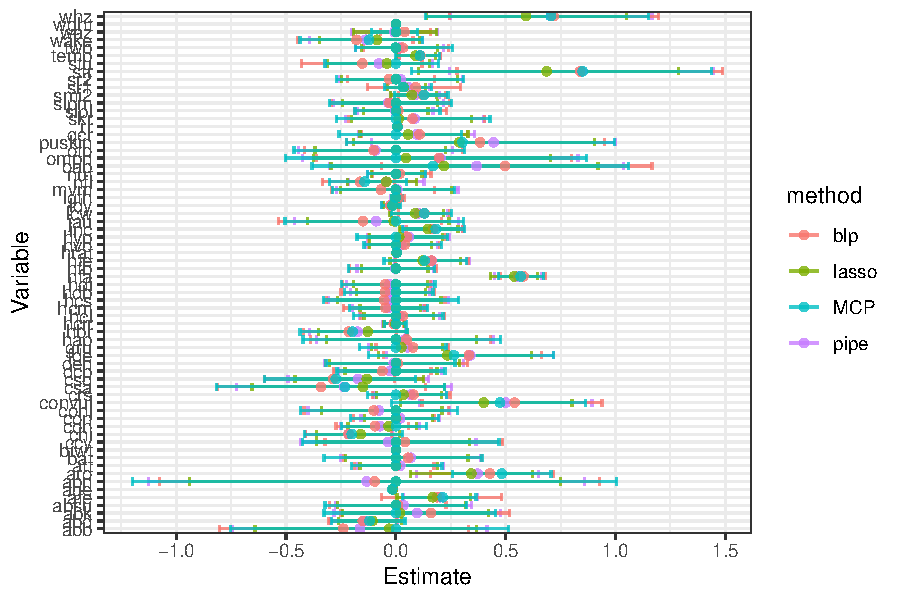
\includegraphics[width=0.6\linewidth]{comparison_data}
  \caption{\label{Fig:comparison_data_whoari} Confidence intervals produced by three different methods for all 66 variables in the \texttt{whoari} dataset ...}
  \end{center}
\end{figure}

\section{Random thoughts / stuff from other papers}

As covered in \logan{cite previous paper}, a simple debiasing procedure only accounts for the first order bias.

That is, for a given variable, it directly accounts for the penalty induced bias but it does not account for the effect the of the bias introduced by biased estimates that a given variable is correlated with. This, what we call second order, bias can still partially be chalked up to the penalty but occurs in a somewhat back door way.

The effect of this bias suggest that the method is not useful, however, the conditions considered in this previous manuscript are not necessarily all that fair. In fact, the main simulation set up considered is primed to highlight this bias. Furthermore, this manuscript also indicated that $\lam_{\CV}$ is not necessarily the best $\lambda$ for the Debiased method.

Additionally as mentioned in that previous manuscript, if one is converned with covering larger magnitude values of $\beta$, then we suggested that the lasso penalty may not be the best option and that the practicioner may one to consider alternative penalties, such as the Minimax Concave Penalty (MCP).

As an extension of these two ideas, we then bring these two streams of thought together and present the debiased method for MCP.

Note that when minimizing CVE, we are not necessarily minimizing the bias of the estimates... but rather the error in the holdout set. Estimating the bias is a much more difficult task

\begin{itemize}
\item \textbf{Debiased bootstrap:} Uses the correlation between $\boldsymbol{\x}^b_j$ and the partial residuals obtained from the model for each bootstrap sample as the bootstrap draw for variable j.
\end{itemize}

Regardless, although Debiased does reduce the rate of intervals missing toward zero for larger magnitude $\beta$s, it is unable to correct all the bias, still missing below at a rater higher than ideal.

The primary point to note for Debiased is that the value f $\lambda$ that produces closest to nominal coverage is outside of the range of $\lambda$s selected by CV. Furthermore, this value occurs at a place that appears to produce nominal coverage across the range of $\beta$ values. As will be covered in the Discussion, the bias of $z_j$ is directly related to the bias of $\bbh_{-j}$. The smaller value of $\lambda$ providing the best performance in this scenario suggests that the performance of Debiased is optimized when $\lam$ is as small as possible to avoid bias explicitly introduced by $\lam$ but large enough to produce a stable estimate for $\bb$. For Debiased, the far left hand side ($\lam_{\max}$) represents marginal regression estimates whereas if $\lam \rightarrow 0$ (towards the right) would be increasingly similar to fully joint estimates for a multiple linear regression model.

This leads to a limitation of the methods proposed here. There is additional bias in the estimates beyond the bias introduced by the penalty. This is most easily observed when considering the debias method but applies to all four methods. Recall that the estimate used for the debiased method is for variable $j$ is $\z_j = \frac{1}{n}\x^T_j \r_j$. As shown in \cite{Breheny2019}, in the non-orthogonal case, 

$$
\frac{1}{n}\x^T_j \r_j = \beta^*_j + \frac{1}{n}\x_j^T \epsilon + \frac{1}{n}\x_j^T \X_{-j}(\bb^*_{-j} - \bbh_{-j}).
$$

Focusing on the last term, this shows that there is bias in $z_j$ from the bias in estimating all other $\bb$s that variable $j$ is correlated with. Of course, $z_j$ is used in the construction of the full conditional posterior and the traditional estimate is essentially $z_j$ with the penalty applied. This indicated that such bias is pervasive in each method. Since this bias depends on the sample correlation, this bias can be present even when features are truly independent. Furthermore, during bootstrap resamples, chance correlation will occur even if the original dataset was generated with orthogonality. That said, this appears not to be considerably detrimental in practice as the methods fare well even with high levels of correlation. Future work could be done to correct this bias, however, consideration should be given estimating this bias for each $\bh_j$ depends on accurately estimating the bias of all other coefficients.

\logan{I actually think the main example (laplace) here is a very severe case in terms of the bias that would be ovserved.}
